
\section{Grading Categories}

% TODO: Find a good reference for this. 
Many Wikipedia articles can be reached from categories that are not describing for the content of the article. We found multiple paths to all Wikipedia articles, but some of them were less descriptive of the content than others. Thus, a grading was done to find the most relevant paths for each article. 

\subsection{Grading based on Inlinks and Outlinks}
%\subsubsection{Inlinks and Outlinks of Categories}
Each category in Wikipedia has a set of parent categories i.e., categories that lead to the current category, and a set of subcategories i.e., categories that can be reached from the current category. The size of these sets for a given category can be annotated as 
\begin{itemize}
\item \emph{Inlink number} = number of parent categories
\item \emph{Outlink number} = number of subcategories
\end{itemize}
Figure \ref{fig:Categorywparentandsub2} is a demonstration of how  inlink and outlink are connected to a category, and gives the idea that a catgory with high \emph{inlink} and \emph{outlink} are more likely to be visited when looking for paths for an article. 

\begin{figure}[h]
\centering
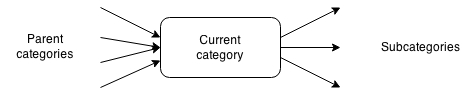
\includegraphics[width=\textwidth]{Chapters/Methods/category_parent_sub}
\caption[Example of \emph{inlink number} and \emph{outlink number} for a category]{Example of how a category has links from parent categories and links to its subcategories. The \emph{inlink number} for the category is 4 and the \emph{outlink number} for the category is 3.}
\label{fig:Categorywparentandsub2}
\end{figure}

Two assumptions can be made from this. The first assumption is that categories with high inlink number can be reached from categories that are not about the same topic. The other assumption is that categories with a high outlink number are more likely to reach articles not necessarily connected to the category name since they can reach far in all the subcategories' directions. Thus, categories with a high value of outlink and a high value of inlink should have a lower score than categories seldom reached. They cover a general topic, while categories with a low inlink number and low outlink number describe a narrow topic.

\subsubsection{Scoring paths}
Grading based on inlinks and outlinks is done by finding the number of inlinks and outlinks for all categories in the structure, and the average number of inlinks and outlinks for all categories. Then the scoring should be weighted based on the values of inlink and outlink which leads to the following equation where $\xoverline{C_{in}}$ is the average \emph{inlink} and $\xoverline{C_{out}}$ is the average \emph{outlink}.  

%The assumption that categories with high \emph{inlink} and \emph{outlink} are more often visited leads to the thought that these categories should have a lower score than categories that are more rarly visited. 

%The first approach was therefore to find the \emph{inlink} and \emph{outlink} of all categories in the structure. These numbers had to be compared with the average number of \emph{inlink} and \emph{outlink} to know whether the number is high or low (see Table \ref{tab:avginlinkoutlink}). 


\begin{equation} \label{eq:categoryscore}
Score_{C} = \frac{inlink_{c} + outlink_{c}}{\xoverline{C_{in}} + \xoverline{C_{out}}}
\end{equation}

This means that the path score of a path $P$ is the sum of the scores of all categories (see equation \ref{eq:scoreinput}). 

\begin{equation} \label{eq:scoreinput}
Pathscore_{P} = \sum_{c} Score_{C}
\end{equation}

The problem with using equation \ref{eq:scoreinput} is that short paths will be favored since there are fewer scores to be added together. A way of avoiding favoritism of short paths is by normalizing the path scores. 

\subsection{Normalized Grading based on Inlink and Outlink Numbers}
Grading based on inlink number and outlink number favors short paths even if the paths contains categories considered as bad. One way of handling this problem is by normalizing the score of each path. Equation \ref{eq:normscoreinput} is a way of normalizing the path score of path $P$ so the length of the path does not determine the relevance of the path. 

% TODO: Write something about normalization - why is it good for grading?

\begin{equation} \label{eq:normscoreinput}
Pathscore_{P} = \frac{1}{N} \sum_{c} Score_{C}
\end{equation}
where $N$ is the number of categories in the path.


\subsection{Deciding Relevant Paths}
One way of deciding which graded paths are relevant are by choosing a threshold for the path score. If the score is lower than a given threshold, it is marked as relevant, while a  higher score means that it is not relevant. A threshold can be found by deciding how many paths should be considered relevant.

One way of doing this is by finding the scores of all paths. and sort the scores from lowest to highest (see \ref{eq:sortedscores}). Then a $k$ has to be decided to how many paths are believed to be relevant of all paths, for instance one could assume that only 10\% of the paths are relevant, which leads to $k = .10 \cdot n$. 

\begin{equation} \label{eq:sortedscores}
Sorted\_scores = \left[ S_{1}, S_{2}, ... , S_{k}, ... , S_{n} \right]
\end{equation}



\begin{equation} \label{eq:threshold}
T = Sorted\_scores[k]
\end{equation}


The problem with this method is that not all articles are guaranteed to have any relevant paths. The other problem is that the score of the path will vary a lot within different fields, since some of the Wikipedia articles are categorized under very specified categories. 
% TODO: Finn en kilde som er enig med meg. 

% Problem: 
% Finne hvor mange pather som er tilgjengelig. 

Another approach is to choose the best $k$ paths for each Wikipedia article. This approach is independent of the values on other articles' path score which means all Wikipedia articles are guaranteed at least one path. The disadvantage is that some paths might be marked as relevant even though their path score is lower than path scores marked as irrelevant by other articles. Another disadvantage is that articles with many good paths will still have to choose the best $k$ paths and good paths might be lost. 

\begin{comment}
Fordeler: ser ikke på de andre
alle articler får minst en score. 

Ulemper: mange gode - hvilken er best?
Kan ikke vite om scoren er god

\end{comment}